\documentclass[aspectratio=43,10pt]{beamer}

% ============================================================
% SOC ASSISTANT — editable Beamer template inspired by supplied PDF
% Compile with pdfLaTeX in Overleaf.
% Optional logo: upload your institute logo as sitlogo.png.
% ============================================================

\usepackage[utf8]{inputenc}
\usepackage[T1]{fontenc}
\usepackage{lmodern}
\usepackage{graphicx}
\usepackage{xcolor}
\usepackage{tikz}
\usetikzlibrary{calc,positioning,arrows.meta,shadows,fit}
\usepackage{booktabs}
\usepackage{colortbl}
\usepackage{tabularx}
\usepackage{array}
\usepackage{ragged2e}

\definecolor{SOCteal}{RGB}{17,94,119}
\definecolor{SOCtealLight}{RGB}{53,145,160}
\definecolor{SOCnav}{RGB}{64,64,64}
\definecolor{SOCdark}{RGB}{19,51,72}
\definecolor{SOCpale}{RGB}{237,243,247}
\definecolor{SOCline}{RGB}{207,219,225}
\definecolor{SOCgray}{RGB}{93,108,118}
\definecolor{SOCwhite}{RGB}{255,255,255}

\usetheme{default}
\setbeamersize{text margin left=0.075\paperwidth,text margin right=0.075\paperwidth}
\setbeamerfont{normal text}{size=\small}
\setbeamercolor{normal text}{fg=SOCdark,bg=white}
\setbeamercolor{structure}{fg=SOCteal}
\setbeamercolor{itemize item}{fg=SOCteal}
\setbeamercolor{itemize subitem}{fg=SOCtealLight}
\setbeamertemplate{navigation symbols}{}
\setbeamertemplate{itemize item}{\raisebox{0.15ex}{\tiny$\blacktriangleright$}}
\setbeamertemplate{itemize subitem}{\raisebox{0.15ex}{\tiny$\blacktriangleright$}}

% Top progress/navigation strip, similar to the PDF
\newcommand{\SOCnavstrip}{%
\begin{tikzpicture}[remember picture,overlay]
  \fill[SOCnav] (current page.north west) rectangle
       ([yshift=-0.34cm]current page.north east);
  \node[anchor=north west,inner sep=0pt,font=\fontsize{4.6}{5.2}\selectfont,
        text=white] at ([xshift=0.12cm,yshift=-0.06cm]current page.north west)
  {Introduction\quad Objectives\quad Motivation\quad Existing Work\quad Related Work\quad Research Gap\quad Methodology\quad Expected Impact\quad Phase 2 Plan\quad Conclusion\quad References};
  \node[anchor=north west,inner sep=0pt,font=\fontsize{4.6}{5.2}\selectfont,
        text=white] at ([xshift=0.12cm,yshift=-0.20cm]current page.north west)
  {$\bullet\bullet\bullet\quad\bullet\bullet\quad\bullet\bullet\quad\bullet\bullet\quad\bullet\bullet\quad\bullet\bullet\quad\bullet\bullet\quad\bullet\bullet\quad\bullet\bullet\quad\bullet\bullet\quad\bullet\bullet$};
\end{tikzpicture}%
}

% Footer strip
\newcommand{\SOCfooter}[1]{%
\begin{tikzpicture}[remember picture,overlay]
  \fill[SOCnav] (current page.south west) rectangle
       ([yshift=0.28cm]current page.south east);
  \node[anchor=west,text=white,font=\fontsize{5.5}{6}\selectfont]
    at ([xshift=0.12cm,yshift=0.14cm]current page.south west)
    {Silicon Institute of Technology};
  \node[anchor=center,text=white,font=\fontsize{5.5}{6}\selectfont]
    at ([yshift=0.14cm]current page.south)
    {AI-Powered SOC Assistant};
  \node[anchor=east,text=white,font=\fontsize{5.5}{6}\selectfont]
    at ([xshift=-0.70cm,yshift=0.14cm]current page.south east)
    {August 19, 2026};
  \node[anchor=east,text=white,font=\fontsize{5.5}{6}\selectfont]
    at ([xshift=-0.10cm,yshift=0.14cm]current page.south east)
    {#1 / 28};
\end{tikzpicture}%
}

% Content-slide heading bar
\newcommand{\SOCheading}[1]{%
\begin{tikzpicture}[remember picture,overlay]
  \fill[SOCteal] (current page.north west) rectangle
       ([yshift=-0.72cm]current page.north east);
  \node[anchor=west,text=white,font=\sffamily\fontsize{15}{17}\selectfont]
    at ([xshift=0.25cm,yshift=-0.36cm]current page.north west) {#1};
\end{tikzpicture}%
}

% Standard content slide
\newcommand{\SOCslide}[2]{%
\begin{frame}[plain]
\SOCnavstrip
\SOCheading{#1}
\vspace*{0.62cm}
#2
\SOCfooter{\thepage}
\end{frame}
}

% Pale card with top rule
\newcommand{\SOCcard}[3]{%
\begin{tikzpicture}
\node[
  draw=SOCline,fill=SOCpale,rounded corners=2pt,
  line width=0.45pt,top color=SOCpale,bottom color=white,
  text width={\dimexpr#1-14pt\relax},inner sep=7pt,align=left,
  drop shadow={opacity=.12,shadow xshift=1pt,shadow yshift=-1pt}
] (card) {\textbf{\color{SOCdark}#2}\\[2pt]\small #3};
\draw[SOCteal,line width=2pt] (card.north west)--(card.north east);
\end{tikzpicture}%
}

% Section divider slide with subtle grid and abstract connector line
\newcommand{\SOCdivider}[2]{%
\begin{frame}[plain]
\SOCnavstrip
\begin{tikzpicture}[remember picture,overlay]
  \fill[white] (current page.south west) rectangle (current page.north east);
  \foreach \x in {0.5,1,...,12.5}
    \draw[ SOCline!35, line width=0.25pt]
      ([xshift=\x cm]current page.south west) -- ([xshift=\x cm]current page.north west);
  \foreach \y in {0.5,1,...,8}
    \draw[ SOCline!30, line width=0.25pt]
      ([yshift=\y cm]current page.south west) -- ([yshift=\y cm]current page.south east);
  \draw[SOCteal!12,line width=1pt]
    ([xshift=-0.2cm,yshift=-3.3cm]current page.west) --
    ([xshift=2.8cm,yshift=-3.3cm]current page.west) --
    ([xshift=4.2cm,yshift=-1.9cm]current page.west) --
    ([xshift=8.3cm,yshift=-1.9cm]current page.west);
  \fill[SOCteal!15] ([xshift=8.3cm,yshift=-1.9cm]current page.west) circle (2pt);
  \draw[SOCteal!12,line width=1pt]
    ([xshift=-0.2cm,yshift=-5.1cm]current page.west) --
    ([xshift=3.2cm,yshift=-5.1cm]current page.west) --
    ([xshift=4.6cm,yshift=-3.7cm]current page.west);
  \node[fill=SOCteal,text=white,rounded corners=4pt,
        minimum width=0.82\paperwidth,minimum height=1.0cm,
        font=\sffamily\Large,drop shadow={opacity=.35,shadow xshift=2pt,shadow yshift=-3pt}]
    at ([yshift=-0.51\paperheight]current page.center) {#1};
  \node[anchor=south east,align=right,text=SOCteal,font=\sffamily\bfseries\Large]
    at ([xshift=-0.55cm,yshift=0.83cm]current page.south east)
    {\IfFileExists{sitlogo.png}{
\includegraphics[width=2.4cm]{sitlogo.png}}{Silicon}};
  \node[anchor=south east,text=SOCgray,font=\scriptsize]
    at ([xshift=-0.55cm,yshift=0.57cm]current page.south east)
    {\IfFileExists{sitlogo.png}{}{...beyond teaching}};
\end{tikzpicture}
\SOCfooter{#2}
\end{frame}
}

\begin{document}

% 1 — Title page
\begin{frame}[plain]
\begin{tikzpicture}[remember picture,overlay]
  \fill[white] (current page.south west) rectangle (current page.north east);
  \fill[SOCteal] ([xshift=0.077\paperwidth]current page.north west)
    rectangle ([xshift=-0.077\paperwidth,yshift=-0.23\paperheight]current page.north east);
  \node[text=white,align=center,text width=.80\paperwidth,
        font=\sffamily\bfseries\fontsize{17}{21}\selectfont]
    at ([yshift=-0.115\paperheight]current page.north)
    {AI-Powered Security Operations Center\\(SOC) Assistant Using Large Language\\Models};
  \node[align=center,font=\sffamily\bfseries\large]
    at ([yshift=-0.303\paperheight]current page.north) {Kunal Sanga};
  \node[align=center,text=SOCgray,font=\sffamily\normalsize]
    at ([yshift=-0.342\paperheight]current page.north) {2301341031};
  \node[align=center,font=\sffamily\bfseries\large]
    at ([yshift=-0.397\paperheight]current page.north) {Soumili Ghosh};
  \node[align=center,text=SOCgray,font=\sffamily\normalsize]
    at ([yshift=-0.436\paperheight]current page.north) {231341057};
  \node[align=center,font=\sffamily\bfseries\large]
    at ([yshift=-0.489\paperheight]current page.north) {Bivan Jena};
  \node[align=center,text=SOCgray,font=\sffamily\normalsize]
    at ([yshift=-0.528\paperheight]current page.north) {2301341021};
  \node[align=center,font=\sffamily\bfseries\small]
    at ([yshift=-0.604\paperheight]current page.north)
    {PPD-2 --- Phase 1 Project Representation};
  \node[align=center,text=SOCgray,font=\sffamily\bfseries\small]
    at ([yshift=-0.713\paperheight]current page.north) {SUPERVISED BY};
  \node[align=center,font=\sffamily\bfseries\LARGE]
    at ([yshift=-0.755\paperheight]current page.north) {Miss. Alka Dash};
  \node[align=center,font=\sffamily\normalsize]
    at ([yshift=-0.795\paperheight]current page.north) {Assistant Professor, CSE};
  \node[align=center,font=\sffamily\small]
    at ([yshift=-0.858\paperheight]current page.north)
    {Silicon Institute of Technology, Sambalpur};
  \node[anchor=center] at ([xshift=-0.13\paperwidth,yshift=-0.88\paperheight]current page.north east)
    {\IfFileExists{sitlogo.png}{
\includegraphics[width=.19\paperwidth]{sitlogo.png}}{}};
  \node[align=center,font=\sffamily\Large]
    at ([yshift=-0.951\paperheight]current page.north) {August 19, 2026};
\end{tikzpicture}
\end{frame}

% 2 — Table of contents
\SOCslide{Table of Contents}{
\begin{minipage}{0.68\textwidth}
\begin{enumerate}
\setlength{\itemsep}{7pt}
\item Introduction
\item Objectives
\item Motivation
\item Existing Work
\item Related Work
\item Research Gap
\item Methodology
\item Expected Impact
\item Phase 2 Plan
\item Conclusion
\item References
\end{enumerate}
\end{minipage}
}

% 3 — Introduction divider
\SOCdivider{Introduction}{3}

% 4 — Introduction to SOC
\SOCslide{INTRODUCTION TO SECURITY OPERATIONS CENTER (SOC)}{
\SOCcard{0.83\textwidth}{Security Operations Center (SOC)}{A Security Operations Center (SOC) is a centralized security environment responsible for continuously monitoring an organization's digital infrastructure, detecting potential threats, investigating security alerts, and supporting incident response.}

\vspace{0.35cm}
\begin{columns}[T,onlytextwidth]
\column{0.47\textwidth}
\SOCcard{0.91\linewidth}{SOC MONITORING}{\begin{itemize}\item Security logs \& events\item Network \& endpoint activity\item Cloud \& application events\end{itemize}}
\column{0.47\textwidth}
\SOCcard{0.91\linewidth}{SOC ANALYST}{\begin{itemize}\item Investigates security alerts\item Correlates security information\item Identifies suspicious activity\item Supports incident response\end{itemize}}
\end{columns}
\vspace{0.25cm}
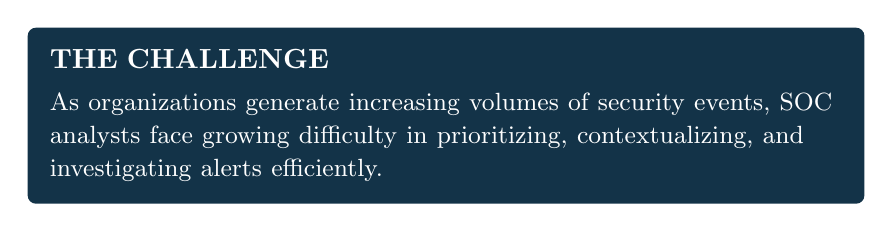
\begin{tikzpicture}
\node[fill=SOCdark,rounded corners=3pt,text=white,text width=.83\textwidth,inner sep=8pt] {
\textbf{THE CHALLENGE}\\[3pt]\small As organizations generate increasing volumes of security events, SOC analysts face growing difficulty in prioritizing, contextualizing, and investigating alerts efficiently.};
\end{tikzpicture}
}

% 5 — Problem statement
\SOCslide{Problem Statement}{
\begin{columns}[T,onlytextwidth]
\column{0.47\textwidth}
\SOCcard{0.92\linewidth}{High Volume of Alerts}{Modern organizations generate huge volumes of security alerts from diverse sources.}
\vspace{0.25cm}
\SOCcard{0.92\linewidth}{Analyst Fatigue}{High alert volume causes fatigue, and manual investigation increases response time.}
\column{0.47\textwidth}
\SOCcard{0.92\linewidth}{Contextual Understanding}{Analysts must determine which alerts are important and represent genuine incidents.}
\vspace{0.25cm}
\SOCcard{0.92\linewidth}{Inconsistent Analysis}{Security analysis can vary according to analyst expertise, affecting quality.}
\end{columns}
\vspace{0.3cm}
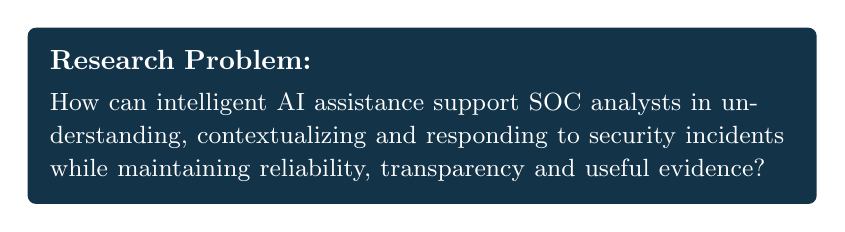
\begin{tikzpicture}
\node[fill=SOCdark,rounded corners=3pt,text=white,text width=.78\textwidth,inner sep=8pt]{
\textbf{Research Problem:}\\[3pt]\small How can intelligent AI assistance support SOC analysts in understanding, contextualizing and responding to security incidents while maintaining reliability, transparency and useful evidence?};
\end{tikzpicture}
}

% 6 — Objectives divider
\SOCdivider{Objectives}{6}

% 7 — Research objectives
\SOCslide{RESEARCH OBJECTIVES}{
\begin{columns}[T,onlytextwidth]
\column{0.47\textwidth}
\begin{itemize}
\setlength{\itemsep}{10pt}
\item \textbf{Identify}\\Key challenges faced by SOC analysts in handling large volumes of security alerts.
\item \textbf{Study}\\Existing AI/ML, LLM and RAG-based approaches for cybersecurity assistance.
\item \textbf{Investigate}\\Approaches for improving contextual understanding and evidence-grounded security analysis.
\end{itemize}
\column{0.47\textwidth}
\begin{itemize}
\setlength{\itemsep}{10pt}
\item \textbf{Explore}\\How intelligent assistance can support SOC analysts while retaining human oversight.
\item \textbf{Establish}\\Suitable criteria for evaluating the effectiveness and reliability of such assistance.
\end{itemize}
\end{columns}
}

% 8 — Motivation divider
\SOCdivider{Motivation}{8}

% 9 — Research motivation
\SOCslide{Research Motivation}{
\begin{columns}[T,onlytextwidth]
\column{0.47\textwidth}
\SOCcard{0.92\linewidth}{Alert Volume}{Large numbers of security events make prioritization and investigation difficult.}
\vspace{0.25cm}
\SOCcard{0.92\linewidth}{Analyst Dependency}{Interpreting complex alerts requires highly specialized cybersecurity knowledge.}
\column{0.47\textwidth}
\SOCcard{0.92\linewidth}{Response Time}{Delayed analysis can slow down incident investigation and response.}
\vspace{0.25cm}
\SOCcard{0.92\linewidth}{Intelligent Assistance}{AI can support repetitive tasks and help analysts access relevant knowledge.}
\end{columns}
\vspace{0.3cm}
\SOCcard{0.83\textwidth}{Potential Impact}{\begin{itemize}\item Faster initial incident understanding and reduced repetitive investigation effort.\item Better access to cybersecurity context and more consistent incident analysis.\end{itemize}}
}

% 10 — Existing work divider
\SOCdivider{Existing Work}{10}

% 11 — Existing work / state of art
\SOCslide{Existing Work / State of the Art}{
\begin{columns}[T,onlytextwidth]
\column{0.31\textwidth}
\SOCcard{0.92\linewidth}{TRADITIONAL SOC}{\begin{itemize}\item Rule-based\item SIEM systems\item Signatures\item Manual triage\end{itemize}}
\column{0.31\textwidth}
\SOCcard{0.92\linewidth}{ML-BASED SECURITY}{\begin{itemize}\item Classification\item Anomaly detection\item Prioritization\item Event analysis\end{itemize}}
\column{0.31\textwidth}
\SOCcard{0.92\linewidth}{LLM-BASED RESEARCH}{\begin{itemize}\item Log analysis\item Threat intel\item Investigation\item Response support\end{itemize}}
\end{columns}
\vspace{0.45cm}
\SOCcard{0.83\textwidth}{Retrieval-Augmented Generation (RAG)}{RAG allows an LLM to access relevant external/domain-specific information before generating a response, providing essential cybersecurity context.}
}

% 12 — Related work divider
\SOCdivider{Related Work}{12}

% 13 — Research papers 1
\SOCslide{Research Papers Reviewed (1/2)}{
\small
\renewcommand{\arraystretch}{1.5}
\begin{tabularx}{\textwidth}{>{\raggedright\arraybackslash}X p{0.10\textwidth} >{\raggedright\arraybackslash}p{0.30\textwidth}}
\toprule
\rowcolor{SOCpale}\textbf{Paper Title \& Venue} & \textbf{Year} & \textbf{Main Relevance}\\
\midrule
Enhancing Security Operations Center: Wazuh Security Event Response with RAG-Driven Copilot (\textit{Sensors}) & 2025 & Security event response, RAG, and analyst assistance. Closest work.\\
\midrule
Large Language Models for Security Operations Centers: A Comprehensive Survey (\textit{Journal of Electrical and Computer Engineering}) & 2026 & Comprehensive survey of LLM applications in SOC workflows.\\
\bottomrule
\end{tabularx}
}

% 14 — Research papers 2
\SOCslide{Research Papers Reviewed (2/2)}{
\small
\renewcommand{\arraystretch}{1.5}
\begin{tabularx}{\textwidth}{>{\raggedright\arraybackslash}X p{0.10\textwidth} >{\raggedright\arraybackslash}p{0.30\textwidth}}
\toprule
\rowcolor{SOCpale}\textbf{Paper Title \& Venue} & \textbf{Year} & \textbf{Main Relevance}\\
\midrule
Evidence-First Retrieval Augmented Generation with Claim Repair for SOC Workflows (\textit{IEEE ICHORA}) & 2026 & Evidence grounding, claim verification and reliable security analysis.\\
\midrule
Non-Disruptive Disruption: An Empirical Experience of Introducing LLMs in the SOC (\textit{NDSS / Internet Society}) & 2026 & Human-AI collaboration and operational SOC workflows.\\
\bottomrule
\end{tabularx}
}

% 15 — Key findings
\SOCslide{KEY FINDINGS FROM LITERATURE SURVEY}{
\begin{columns}[T,onlytextwidth]
\column{0.47\textwidth}
\begin{itemize}
\setlength{\itemsep}{10pt}
\item \textbf{LLM Integration}\\LLMs are increasingly being explored for SOC workflows.
\item \textbf{RAG Utility}\\RAG provides domain-specific cybersecurity context to LLMs.
\item \textbf{Stronger Grounding}\\Security analysis requires stronger grounding than standard chat.
\end{itemize}
\column{0.47\textwidth}
\begin{itemize}
\setlength{\itemsep}{10pt}
\item \textbf{Remaining Challenges}\\Alert classification, context, and response remain challenging.
\item \textbf{Human-in-the-Loop}\\Human analysts remain vital for validating high-impact decisions.
\item \textbf{Limited Novelty}\\A generic cybersecurity chatbot alone would provide limited novelty.
\end{itemize}
\end{columns}
}

% 16 — Research gap divider
\SOCdivider{Research Gap}{16}

% 17 — Preliminary research gap
\SOCslide{Preliminary Research Gap}{
\textbf{Existing Research:}\\
LLM-based SOC assistance is feasible and promising. However, challenges remain in:

\vspace{0.35cm}
\begin{columns}[T,onlytextwidth]
\column{0.31\textwidth}
\SOCcard{0.92\linewidth}{Trust \& Grounding}{Evidence reliability of generated claims.}
\column{0.31\textwidth}
\SOCcard{0.92\linewidth}{Response Quality}{Actionability and recommendation quality.}
\column{0.31\textwidth}
\SOCcard{0.92\linewidth}{Methodology}{Evaluation methodology and integration.}
\end{columns}
\vspace{0.5cm}
\SOCcard{0.83\textwidth}{Research Opportunity}{Investigate how AI-assisted SOC analysis can provide more reliable and context-aware incident support while keeping supporting evidence visible to the analyst.}
}

% 18 — Methodology divider
\SOCdivider{Methodology}{18}

% 19 — High-level methodology
\SOCslide{HIGH-LEVEL METHODOLOGY}{
\begin{center}
\small High-level research workflow --- detailed implementation in Phase 2
\vspace{0.35cm}

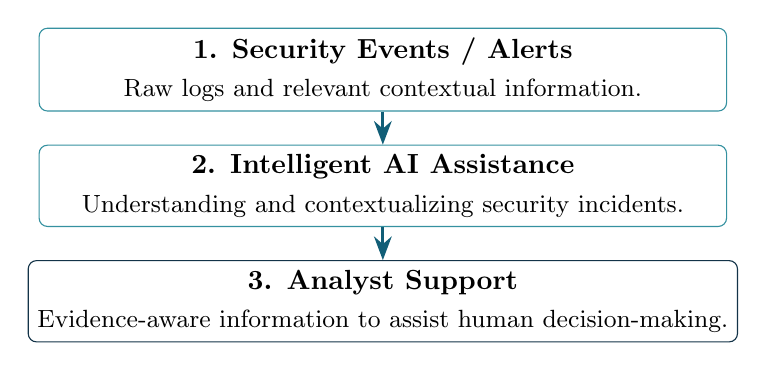
\begin{tikzpicture}[node distance=0.42cm]
\node[draw=SOCtealLight,rounded corners=3pt,minimum width=.72\textwidth,minimum height=0.9cm,align=center,fill=white] (a)
{\textbf{1. Security Events / Alerts}\\[2pt]\small Raw logs and relevant contextual information.};
\node[draw=SOCtealLight,rounded corners=3pt,minimum width=.72\textwidth,minimum height=0.9cm,align=center,fill=white,below=of a] (b)
{\textbf{2. Intelligent AI Assistance}\\[2pt]\small Understanding and contextualizing security incidents.};
\node[draw=SOCdark,rounded corners=3pt,minimum width=.72\textwidth,minimum height=0.9cm,align=center,fill=white,below=of b] (c)
{\textbf{3. Analyst Support}\\[2pt]\small Evidence-aware information to assist human decision-making.};
\draw[-{Stealth[length=3mm]},line width=1pt,SOCteal] (a.south)--(b.north);
\draw[-{Stealth[length=3mm]},line width=1pt,SOCteal] (b.south)--(c.north);
\end{tikzpicture}

\vspace{0.2cm}
\textbf{\color{SOCgray}Detailed methodology and implementation will be presented in Phase 2.}
\end{center}
}

% 20 — Expected impact divider
\SOCdivider{Expected Impact}{20}

% 21 — Impact and evaluation
\SOCslide{Expected Impact \& Evaluation Direction}{
\begin{columns}[T,onlytextwidth]
\column{0.47\textwidth}
\SOCcard{0.92\linewidth}{Potential Impact}{\begin{itemize}\item Faster incident understanding\item Reduced repetitive effort\item Improved access to context\item More consistent explanations\item Better analyst decision support\end{itemize}}
\column{0.47\textwidth}
\SOCcard{0.92\linewidth}{Potential Evaluation Dimensions}{\begin{itemize}\item \textbf{Detection:} Accuracy, Precision, F1\item \textbf{Retrieval:} Relevance and coverage\item \textbf{Reliability:} Evidence grounding\item \textbf{Response:} Correctness \& actionability\item \textbf{Efficiency:} Time and latency\end{itemize}}
\end{columns}
}

% 22 — Phase 2 plan divider
\SOCdivider{Phase 2 Plan}{22}

% 23 — Planned research work
\SOCslide{Phase 2 --- Planned Research Work}{
\begin{center}
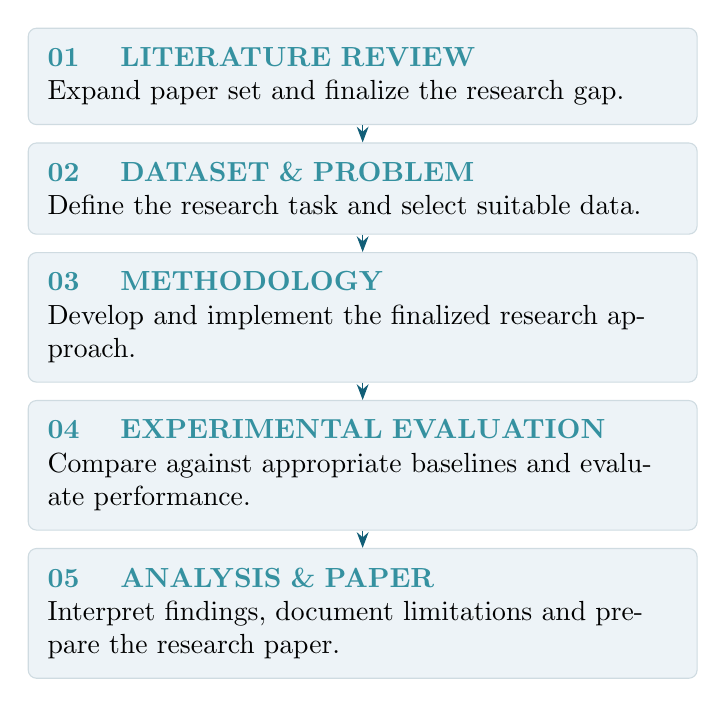
\begin{tikzpicture}[node distance=0.22cm]
\node[draw=SOCline,fill=SOCpale,rounded corners=3pt,text width=.66\textwidth,inner sep=7pt] (a)
{\textbf{\color{SOCtealLight}01 \quad LITERATURE REVIEW}\\Expand paper set and finalize the research gap.};
\node[draw=SOCline,fill=SOCpale,rounded corners=3pt,text width=.66\textwidth,inner sep=7pt,below=of a] (b)
{\textbf{\color{SOCtealLight}02 \quad DATASET \& PROBLEM}\\Define the research task and select suitable data.};
\node[draw=SOCline,fill=SOCpale,rounded corners=3pt,text width=.66\textwidth,inner sep=7pt,below=of b] (c)
{\textbf{\color{SOCtealLight}03 \quad METHODOLOGY}\\Develop and implement the finalized research approach.};
\node[draw=SOCline,fill=SOCpale,rounded corners=3pt,text width=.66\textwidth,inner sep=7pt,below=of c] (d)
{\textbf{\color{SOCtealLight}04 \quad EXPERIMENTAL EVALUATION}\\Compare against appropriate baselines and evaluate performance.};
\node[draw=SOCline,fill=SOCpale,rounded corners=3pt,text width=.66\textwidth,inner sep=7pt,below=of d] (e)
{\textbf{\color{SOCtealLight}05 \quad ANALYSIS \& PAPER}\\Interpret findings, document limitations and prepare the research paper.};
\foreach \x/\y in {a/b,b/c,c/d,d/e}
\draw[-{Stealth[length=2mm]},SOCteal] (\x.south)--(\y.north);
\end{tikzpicture}
\end{center}
}

% 24 — Conclusion divider
\SOCdivider{Conclusion}{24}

% 25 — Conclusion
\SOCslide{Conclusion}{
\begin{itemize}
\setlength{\itemsep}{9pt}
\item SOC environments face increasing alert volume and investigation complexity.
\item Existing research shows growing interest in LLM-based cybersecurity assistance.
\item Literature indicates that reliability, evidence grounding and human-AI collaboration remain important challenges.
\item A preliminary research opportunity has been identified to improve reliability and context-awareness.
\item Detailed methodology and experimental implementation will be developed in Phase 2.
\end{itemize}
}

% 26 — References divider
\SOCdivider{References}{26}

% 27 — References
\SOCslide{References}{
\small
\begin{enumerate}
\setlength{\itemsep}{9pt}
\item Ismail et al., ``Enhancing Security Operations Center: Wazuh Security Event Response with Retrieval-Augmented-Generation-Driven Copilot'', \textit{Sensors}, 2025.
\item Habibzadeh, Feyzi \& Ebrahimi Atani, ``Large Language Models for Security Operations Centers: A Comprehensive Survey'', \textit{Journal of Electrical and Computer Engineering}, 2026.
\item Taysi et al., ``Evidence-First Retrieval Augmented Generation with Claim Repair for Security Operations Center Workflows'', \textit{IEEE ICHORA}, 2026.
\item Hahn et al., ``Non-Disruptive Disruption: An Empirical Experience of Introducing LLMs in the SOC'', \textit{NDSS / Internet Society}, 2026.
\end{enumerate}
}

% 28 — Thank you
\begin{frame}[plain]
\SOCnavstrip
\begin{tikzpicture}[remember picture,overlay]
  \fill[white] (current page.south west) rectangle (current page.north east);
  \node[align=center,font=\sffamily\bfseries\Huge,text=SOCteal]
    at ([yshift=-0.43\paperheight]current page.north) {Thank You};
  \node[align=center,font=\sffamily\Large,text=SOCdark]
    at ([yshift=-0.51\paperheight]current page.north) {Questions \& Discussion};
  \node[anchor=south east,text=SOCteal,font=\sffamily\bfseries\Large]
    at ([xshift=-0.55cm,yshift=0.83cm]current page.south east)
    {\IfFileExists{sitlogo.png}{
\includegraphics[width=2.4cm]{sitlogo.png}}{Silicon}};
\end{tikzpicture}
\SOCfooter{28}
\end{frame}

\end{document}